% =============================================================================
\section{Cómo habla ROS 2 con PX4}
% =============================================================================

\begin{frame}{El puente: uXRCE-DDS}
  \centering
  \begin{tikzpicture}[node distance=0.4cm,every node/.style={font=\scriptsize},
      bx/.style={draw=azul,fill=azulclaro,rounded corners,minimum height=1cm,minimum width=2.4cm,align=center}]
    \node[bx] (u) {uORB\\(dentro de PX4)};
    \node[bx,right=0.6cm of u] (c) {uxrce\_dds\_client\\(módulo de PX4)};
    \node[bx,right=1.4cm of c] (a) {MicroXRCEAgent\\(en la computadora)};
    \node[bx,right=0.6cm of a,fill=yellow!20] (r) {topics de ROS 2\\/fmu/in, /fmu/out};
    \draw[{Stealth}-{Stealth}] (u) -- (c);
    \draw[{Stealth}-{Stealth},thick] (c) -- node[above]{XRCE} node[below,font=\tiny]{UDP o serial} (a);
    \draw[{Stealth}-{Stealth}] (a) -- node[above]{DDS} (r);
  \end{tikzpicture}
  \vspace{0.6em}
  \begin{itemize}\small
    \item DDS ``completo'' es pesado para una controladora: PX4 habla \textbf{XRCE-DDS}, la versión para
      microcontroladores.
    \item El \textbf{agente} traduce a DDS normal: del otro lado ROS 2 ve topics comunes y corrientes.
    \item Sin agente corriendo, \textbf{no hay ningún topic de PX4} en ROS 2.
    \item SITL: \cmd{MicroXRCEAgent udp4 -p 8888}. Dron real: por serial (\cmd{vespo up --real}).
  \end{itemize}
\end{frame}

\begin{frame}{El diagrama oficial}
  \centering
  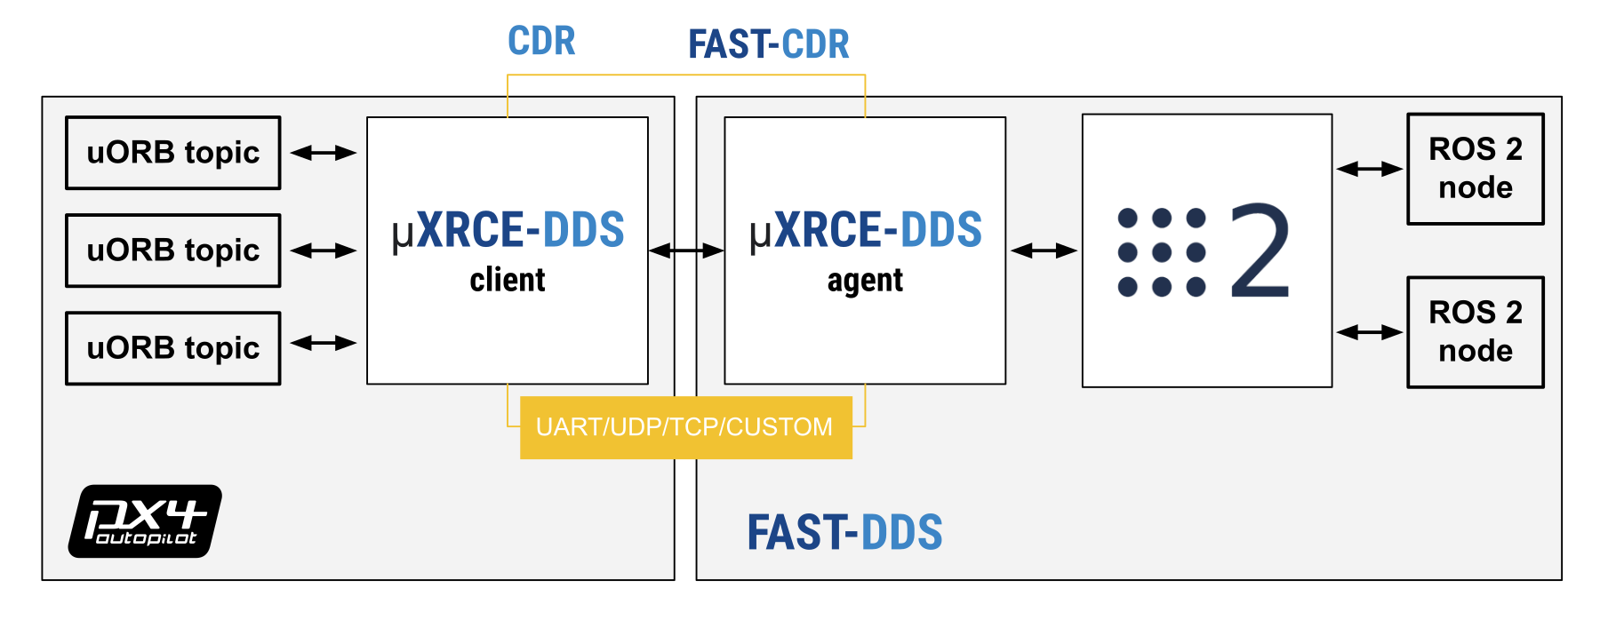
\includegraphics[width=0.95\linewidth]{xrce_dds}\\
  \credito{Arquitectura de uXRCE-DDS. Documentación de PX4 (CC BY 4.0)}
  \vspace{0.4em}

  \raggedright\small A la izquierda los topics uORB dentro de PX4; en medio el cliente (en PX4) y el agente (en la
  computadora) unidos por UART, UDP o TCP; a la derecha los nodos de ROS 2.
\end{frame}

\begin{frame}{/fmu/out y /fmu/in}
  \begin{columns}[t]
    \column{0.48\textwidth}
    \begin{idea}[title={\small\bfseries /fmu/out/\ldots: PX4 nos cuenta},coltitle=black,colbacktitle=azulclaro]
      \scriptsize
      \cmd{vehicle\_status\_v1}\\
      \cmd{vehicle\_local\_position\_v1}\\
      \cmd{vehicle\_global\_position}\\
      \cmd{vehicle\_attitude}\\
      \cmd{sensor\_combined}\\
      \cmd{vehicle\_gps\_position}\\
      \cmd{battery\_status\_v1}\\
      \cmd{home\_position\_v1}\\
      \cmd{failsafe\_flags}\\
      \cmd{vehicle\_command\_ack}
    \end{idea}
    \column{0.48\textwidth}
    \begin{idea}[title={\small\bfseries /fmu/in/\ldots: le pedimos a PX4},coltitle=black,colbacktitle=azulclaro]
      \scriptsize
      \cmd{offboard\_control\_mode}\\
      \cmd{trajectory\_setpoint}\\
      \cmd{vehicle\_command}
    \end{idea}
    \vspace{0.4em}\small
    Solo existen los topics que PX4 decide exponer: la lista está en
    \cmd{src/modules/uxrce\_dds\_client/dds\_topics.yaml} de PX4 (con su frecuencia máxima).
  \end{columns}
\end{frame}

\begin{frame}[fragile]{dds\_topics.yaml}
  \begin{lstlisting}[language=yaml,caption={Un pedazo del archivo de PX4 v1.17}]
publications:
  - topic: /fmu/out/battery_status
    type: px4_msgs::msg::BatteryStatus
    rate_limit: 1.            # a 1 Hz como mucho
  - topic: /fmu/out/vehicle_attitude
    type: px4_msgs::msg::VehicleAttitude
subscriptions:
  - topic: /fmu/in/trajectory_setpoint
    type: px4_msgs::msg::TrajectorySetpoint
  - topic: /fmu/in/vehicle_command
    type: px4_msgs::msg::VehicleCommand
  \end{lstlisting}
  \small Si un ejemplo no recibe nada, lo primero es revisar que el topic esté aquí y que el nombre sea
  exacto (incluido el sufijo de versión).
\end{frame}

\begin{frame}{Los sufijos \_v1: versiones de mensajes}
  \begin{columns}[c]
    \column{0.55\textwidth}\small
    Cuando PX4 cambia los campos de un mensaje, sube su \cmd{MESSAGE\_VERSION} y el topic cambia de nombre:
    \begin{center}\scriptsize
      \begin{tabular}{lcl}
        \toprule
        Mensaje & versión & topic \\
        \midrule
        \cmd{VehicleStatus} & 1 & \cmd{vehicle\_status\_v1} \\
        \cmd{VehicleLocalPosition} & 1 & \cmd{vehicle\_local\_position\_v1} \\
        \cmd{BatteryStatus} & 1 & \cmd{battery\_status\_v1} \\
        \cmd{HomePosition} & 1 & \cmd{home\_position\_v1} \\
        \cmd{VehicleGlobalPosition} & 0 & \cmd{vehicle\_global\_position} \\
        \cmd{VehicleAttitude} & 0 & \cmd{vehicle\_attitude} \\
        \bottomrule
      \end{tabular}
    \end{center}
    Versión 0 = sin sufijo.
    \column{0.42\textwidth}
    \begin{ojo}
      \small Si te suscribes a \cmd{/fmu/out/vehicle\_status} (sin \cmd{\_v1}) \textbf{no llega nada} y no hay
      ningún error: simplemente nadie publica en ese nombre.
    \end{ojo}
  \end{columns}
\end{frame}

\begin{frame}{px4\_msgs tiene que coincidir con PX4}
  \begin{columns}[c]
    \column{0.55\textwidth}\small
    \begin{itemize}
      \item \cmd{px4\_msgs} es un paquete de ROS 2 con los \textbf{mismos .msg} que tu versión de PX4.
      \item Si no coinciden, el agente no puede traducir: los topics ``existen'' pero los datos salen
        mal o no llegan.
      \item Por eso \cmd{vespo.toml} fija la versión de PX4 (v1.17.0) y \cmd{vespo.repos} el commit de
        \cmd{px4\_msgs} (\cmd{release/1.17}).
      \item \cmd{vespo px4 update} mueve los dos juntos.
    \end{itemize}
    \column{0.42\textwidth}\centering
    \begin{tikzpicture}[every node/.style={font=\tiny}]
      \node[draw=azul,fill=azulclaro,rounded corners,align=center] (p) {PX4 v1.17.0\\msg/*.msg};
      \node[draw=azul,fill=azulclaro,rounded corners,align=center,below=1cm of p] (m) {px4\_msgs\\release/1.17};
      \draw[{Stealth}-{Stealth},thick,verde] (p) -- node[right]{iguales} (m);
    \end{tikzpicture}
  \end{columns}
\end{frame}

\begin{frame}{QoS: cómo se entregan los mensajes}
  \small Cada publisher y subscriber de ROS 2 tiene una \textbf{calidad de servicio} (QoS). PX4 publica con:
  \begin{center}
    \cmd{rclcpp::QoS(1).best\_effort().transient\_local()}
  \end{center}
  \centering\scriptsize
  \begin{tabular}{lll}
    \toprule
    Parte & Significa & Por qué \\
    \midrule
    \cmd{QoS(1)} & guardar solo el último mensaje & solo importa el dato más reciente \\
    \cmd{best\_effort} & si se pierde uno, no se reenvía & a 100 Hz el siguiente llega enseguida \\
    \cmd{transient\_local} & al conectarte recibes el último que se publicó & no esperar al siguiente \\
    \bottomrule
  \end{tabular}
  \vspace{0.4em}
  \raggedright
  \begin{ojo}
    \small Un subscriber \cmd{reliable} \textbf{no recibe nada} de un publisher \cmd{best\_effort}. Por eso todos
    los ejemplos crean su suscripción con el mismo QoS que PX4.
  \end{ojo}
\end{frame}

\begin{frame}{Compatibilidad de QoS}
  \centering\small
  \begin{tabular}{llc}
    \toprule
    Publisher & Subscriber & ¿Se conectan? \\
    \midrule
    best\_effort & best\_effort & \ok \\
    reliable & best\_effort & \ok \\
    reliable & reliable & \ok \\
    best\_effort & reliable & \mal{} (nunca llega nada) \\
    \bottomrule
  \end{tabular}
  \vspace{0.6em}

  \raggedright\small
  \begin{itemize}
    \item Regla: el subscriber puede pedir \textbf{menos} que lo que ofrece el publisher, nunca más.
    \item Entre nodos nuestros (\cmd{battery\_publisher} $\rightarrow$ \cmd{battery\_subscriber}) usamos el
      QoS por defecto (reliable), porque no hace falta otra cosa.
    \item \cmd{ros2 topic info -v /fmu/out/vehicle\_status\_v1} muestra el QoS de cada lado.
  \end{itemize}
\end{frame}

\begin{frame}[fragile]{Timestamps: microsegundos desde que arrancó PX4}
  \small Todos los mensajes de PX4 empiezan con \cmd{uint64 timestamp}: tiempo desde que arrancó el sistema,
  en \textbf{microsegundos}.
  \begin{lstlisting}[style=cpp,caption={Así ponen el timestamp los ejemplos al publicar}]
uint64_t now_us() {
  return get_clock()->now().nanoseconds() / 1000;   // ns -> us
}
msg.timestamp = now_us();
  \end{lstlisting}
  \begin{itemize}
    \item Si un mensaje recibido tiene \cmd{timestamp == 0}, \textbf{todavía no ha llegado ninguno} (los
      mensajes nacen con todos sus campos en 0). \cmd{telemetry\_listener} lo usa para avisar.
    \item PX4 sincroniza su reloj con el del agente; en la práctica basta con mandar el tiempo actual.
  \end{itemize}
\end{frame}

\begin{frame}[fragile]{Explorar desde la terminal}
  \begin{lstlisting}[style=bash,caption={Con el agente y PX4 corriendo}]
ros2 topic list | grep fmu                            # qué expone PX4
ros2 topic echo /fmu/out/vehicle_status_v1 --once     # un mensaje
ros2 topic hz /fmu/out/sensor_combined                # qué tan rápido llega
ros2 interface show px4_msgs/msg/VehicleCommand       # los campos de un tipo
ros2 topic info -v /fmu/out/vehicle_local_position_v1 # QoS de cada lado
  \end{lstlisting}
  \begin{terminal}{ros2 topic echo /fmu/out/vehicle\_status\_v1 --field nav\_state}
14\\
---\\
14
  \end{terminal}
\end{frame}
